\documentclass[11pt]{article}
\usepackage[letterpaper,margin=1in]{geometry}
\usepackage[T1]{fontenc}
\usepackage{mathptmx}
\usepackage{amsmath,amssymb,amsthm}
\usepackage{graphicx}
\usepackage{booktabs}
\usepackage{threeparttable}
\usepackage[font=small,labelfont=bf]{caption}
\usepackage[numbers,sort&compress]{natbib}
\usepackage{xcolor}
\usepackage{microtype}
\usepackage{authblk}
\usepackage[colorlinks=true,linkcolor=blue!50!black,citecolor=blue!50!black,urlcolor=blue!50!black]{hyperref}
\renewcommand{\baselinestretch}{1.12}
\setlength{\emergencystretch}{3em}
\newcommand{\chitwo}{\chi^{(2)}}
\newcommand{\aw}{\alpha_{\omega}}
\newcommand{\aww}{\alpha_{2\omega}}
\newcommand{\Et}{\tilde E}
\let\hbar\relax\DeclareRobustCommand{\hbar}{{\mathchar'26\mkern-9mu h}}
\newtheorem{proposition}{Proposition}

\title{Depolarization beyond energy shifts: pathway factors, multisubband coupling and dynamic screening in resonant intersubband second-harmonic generation}
\author{Gracen Ownby}
\affil{University of Oklahoma, Norman, Oklahoma, USA}
\date{\small 20 October 2026}

\begin{document}
\maketitle

\begin{abstract}
In doped quantum wells the electrons screen the field that drives them, which blue-shifts each intersubband resonance by the depolarization shift. Second-order susceptibilities of real structures are usually computed in one of two ways: by substituting the shifted energies into the single-particle formula, or by multiplying the bare susceptibility by local-field factors of an effective medium with a single depolarization length. We solve the second-order time-dependent Hartree (random-phase) equations in the subband basis, including the diagonal (permanent-dipole) kernel terms, and compare both shortcuts with the self-consistent response.

To leading order in the rotating-wave approximation each pathway carries its own factor $F_p=1-\kappa_p\Delta_{12}/(\Et_{12}-\hbar\omega-i\gamma)$. Here $\kappa_p$ is a ratio of Hartree overlaps of cumulative transition charges; for the excited-state pathway $\kappa_\mathrm{exc}=c\sqrt{L_{12}/L_{23}}$, where $|c|\le1$ is the shape correlation of the two transition charges and $L_{ij}$ their effective lengths. For the excited-state pathway this is the coupling factor of Załużny's three-level theory, whose GaAs step-well results our solver reproduces; the permanent-dipole Hartree terms he omitted lower his predicted enhancement by 11\%. The solver also reproduces the shift of the optimum double-well design to collective double resonance found by Krieguer and Todorov, with an enhancement of 2.4 against their estimate of almost 3. Energy substitution corresponds approximately to $\kappa=0$ and the single-length effective medium to $\kappa=1$. Real structures lie in between: $\kappa_\mathrm{exc}=0.83$--$0.87$ for asymmetric double wells and 0.54 for a coupled triple well.

Whether the collective terms raise or lower $|\chitwo|$ depends on interference between pathways. With only the ground subband occupied they raise it by 11--38\% at $1$--$2\times10^{12}$~cm$^{-2}$ in an asymmetric double well, but lower it by up to 23\% in the triple well. At room temperature and high density, level 2 of the double well is partly occupied (thermally and by Fermi degeneracy), and the same kernel element couples the 1--2 and 2--3 resonances into a multisubband-plasmon doublet. This lowers the pump absorption by 34\% relative to energy substitution and removes the enhancement; setting $\rho_2=0$ restores a single line and a 38\% enhancement.

For five active regions energy substitution gives the peak $|\chitwo|$ to within 6\% up to $10^{12}$~cm$^{-2}$. At $2\times10^{12}$~cm$^{-2}$ energy substitution errs by up to 18\% in $|\chitwo|$ and the local-field model by up to 20\%; at $4\times10^{12}$~cm$^{-2}$, where upper ladder levels are box-dependent resonances above the spacer band edge, the errors reach a factor of 2 and 37\%. In the optimum-length efficiency merit at double resonance energy substitution errs by up to a factor of 1.6 and the local-field model by up to a factor of 1.4. Feeding measured (already shifted) energies to a local-field model counts the depolarization twice and lowers $|\chitwo|$ by up to 49\%. Under saturation, real-time solutions at $2\times10^{12}$~cm$^{-2}$ give $|\chitwo|$ one third of a frozen-shift rate-model value at 30~MW/cm$^2$. The cause is the static Hartree field of electrons transferred between the wells by the pump: it raises $E_{12}$ by up to 15~meV, brings the 2--3 resonance onto the pump as well, and makes the two population terms of $\chitwo$ partly cancel. Up to 3~MW/cm$^2$ a rate model that includes this field reproduces the real-time $|\chitwo|$ to within 14\%. At $5\times10^{11}$~cm$^{-2}$ the frozen-shift model holds to within 10\%.
\end{abstract}

\section{Introduction}
Resonant intersubband (ISB) transitions give doped quantum wells (QWs) second-order susceptibilities far above those of bulk crystals \cite{Rosencher1991,Rosencher1996,Vurgaftman2021}. They are used both in waveguides \cite{Vurgaftman1996,Vodopyanov1998,Chesi2023,TalamasSimola2024} and in metasurfaces \cite{Lee2014,GomezDiaz2015,Nefedkin2022,Krakofsky2025}.

Large $\chitwo$ needs large electron densities, and at large density the electrons respond collectively: the field acting on an electron includes the Hartree field of the induced charge. In linear response this depolarization effect shifts the ISB resonance from the single-particle energy $E_{12}$ to $\Et_{12}=(E_{12}^2+2E_{12}\Delta_{12})^{1/2}$ \cite{Ando1982}, which is several meV at $10^{12}$~cm$^{-2}$ and routinely seen in absorption \cite{Warburton1996}. When several transitions are close in energy, the collective response couples them into multisubband plasmons that redistribute oscillator strength \cite{Delteil2012}. Under strong excitation the shift depends on intensity \cite{Zaluzny1993}, and it can be removed, ``undressing'' the collective excitation \cite{Craig1996}.

For the nonlinear response two shortcuts are common:
\begin{itemize}
\item \emph{Energy substitution} inserts the shifted energies $\Et_{ij}$, calculated or taken from absorption spectra, into the single-particle density-matrix expression for $\chitwo$ and keeps the bare dipoles \cite{Vurgaftman1996,Vurgaftman2021}.
\item \emph{The effective-medium approach} drives the bare response by a local field, which gives $\chitwo=\Lambda(\omega)^2\Lambda(2\omega)\chitwo_\mathrm{bare}$ with $\Lambda=1/(1+\chi^{(1)}_\mathrm{bare}/\varepsilon_b)$. The same factors appear when the doped layer is described by a single-Lorentzian-per-layer permittivity $\varepsilon_{zz}(\omega)$ in a full-wave calculation; they are the origin of the epsilon-near-zero enhancement of the normal field.
\end{itemize}

Earlier work has studied collective effects in nonlinear ISB optics:
\begin{itemize}
\item Załużny solved the second-order RPA response of a three-level asymmetric step well with the microscopic Coulomb matrix elements, in the rotating-wave approximation and with only the near-resonant terms \cite{Zaluzny1995}. He showed that energy substitution is the ``diagonal approximation'' of that theory, that the coupling between the 1--2 and 2--3 transitions multiplies $\chitwo$ by an additional factor $c(\omega)$, and that in a GaAs step well at $10^{12}$~cm$^{-2}$ this raises the maximum of $|\chitwo|^2$ by a factor of 2.5. For a two-level well he found that depolarization only shifts the SHG peak.
\item Heyman \emph{et al.}\ observed second- and third-harmonic resonances at the depolarization-shifted energy and analysed them with dynamic screening \cite{Heyman1994}.
\item Cominotti \emph{et al.}\ developed a theory of coherent ISB nonlinearities in which strong driving quenches the oscillator strength and suppresses the depolarization shift \cite{Cominotti2023}.
\item Krieguer and Todorov derived $\chitwo$ for collective bright modes coupled by Coulomb terms with normalized overlaps of the transition polarization densities, within a fermionic PZW theory of microcavity-coupled wells \cite{Krieguer2024}. In their theory the dipoles are dressed by the linear response of the other transitions, and the static (population) terms average out because the cavity modes have no in-plane average; they note that these terms do matter in planar geometries. Their three-subband example (GaAs/Al$_{0.3}$Ga$_{0.7}$As double wells, only the ground subband occupied, flat bands, one broadening) couples the 1--2 and 1--3 plasmons and leaves 2--3 at its single-particle energy. They find that at high density the maximum of $|\chitwo|$ moves to designs that are doubly resonant in the collective energies, $\tilde E_{12}\approx\tilde E_{13}/2$, with almost three times the single-particle value, and that in strongly coupled microcavities the efficient designs match polariton states rather than the doubly resonant condition.
\end{itemize}

What remains open, and is our subject, is:
\begin{itemize}
\item when the two shortcuts used in device modelling agree with the self-consistent second-order response of real multilevel structures in a planar geometry, where the diagonal Hartree terms do not average out;
\item why they fail when they do;
\item what this means for the conversion efficiency rather than for $\chitwo$ alone.
\end{itemize}
The last point matters because the optimum-length efficiency of a resonant ladder depends on $|\chitwo|^2/(\aw\aww)$ and on the absorption ratio \cite{OwnbyNL02}, and collective effects change $\chitwo$, $\aw$ and $\aww$ together.

Specifically, we:
\begin{itemize}
\item solve the time-dependent Hartree (TDH, random-phase) equations to second order and in real time;
\item express the result through pathway-resolved factors that contain both shortcuts as limits;
\item relate the couplings to the geometry of the transition charges;
\item identify how partial occupation of the intermediate level limits the collective enhancement in a doubly resonant ladder;
\item show that under saturation the static Hartree field of pump-transferred electrons dominates the corrections to frozen-shift models;
\item quantify the consequences for $|\chitwo|$, absorption and the efficiency merit in five active regions, two of them published;
\item quantify the error of double counting;
\end{itemize}
The calculations use the open-source package qwkit \cite{qwkit}, which contains the TDH module, its tests and the scripts that regenerate every figure and table.

\section{Theory}\label{sec:theory}
\subsection{Time-dependent Hartree equations}
Consider one period of a multiple-QW stack with subbands $|i\rangle$. Each has energy $E_i$, a real envelope function $\psi_i(z)$ and an equilibrium fractional population $\rho^0_i$; $n_s$ is the sheet density. The stack is driven by a $z$-polarized field. Because the normal displacement is continuous, we specify the drive as the field $E_d=D_z/\varepsilon_b$ the stack would carry without the electrons, where $\varepsilon_b$ is a uniform background permittivity. The Hartree potential of the induced charge is then confined to the period.

With the cumulative transition charges
\begin{equation}
F_{ij}(z)=\int_{-\infty}^{z}\psi_i\psi_j\,dz',\qquad S_{ij,kl}=\int F_{ij}(z)F_{kl}(z)\,dz,\label{eq:S}
\end{equation}
the Hartree potential of a density-matrix change $\delta\rho$ has subband matrix elements $[U_H]_{ij}=K\sum_{kl}S_{ij,kl}\,\delta\rho_{kl}$, with $K=q^2n_s/(\varepsilon_0\varepsilon_b)$. Because $F_{ii}(+\infty)=1$, the elements $S_{ii,kl}$ individually depend on the integration range. Only differences such as $S_{22,kl}-S_{11,kl}$ enter physical results, because $\mathrm{Tr}\,\delta\rho=0$ and only differences of diagonal potentials matter.

The density matrix of the conduction subbands obeys
\begin{equation}
\dot\rho=-\frac{i}{\hbar}\big[H_0+qE_d(t)z+U_H[\rho-\rho^0],\rho\big]+\Gamma(\rho-\rho^0),\label{eq:tdh}
\end{equation}
where coherences decay at rate $\gamma/\hbar$ and populations relax through a rate matrix. The polarization is $P=-qN\,\mathrm{Tr}(z\rho)$, where $N$ is the period-averaged volume density. Setting $S=0$ gives the single-particle (bare) equations.

We solve Eq.~\eqref{eq:tdh} in two ways:
\begin{itemize}
\item \emph{Order by order in frequency}, with $E_d=E\,e^{-i\omega t}+\mathrm{c.c.}$ \cite{Boyd2008}. Then $\rho^{(1)}$ and $\rho^{(2)}$ follow from two linear solves of the Liouvillian, which includes $U_H$. The second-order source is $-(i/\hbar)[\tilde U,\rho^{(1)}]$, with the effective first-order potential $\tilde U=qEz+U_H[\rho^{(1)}]$.
\item \emph{In real time}, by fourth-order Runge--Kutta integration of the full nonlinear equation. The harmonics are extracted over an integer number of periods after the populations have settled.
\end{itemize}

For a single transition the linear solution reproduces Ando's shift $\Et_{12}^2=E_{12}^2+2E_{12}\Delta_{12}$ \cite{Ando1982}, with
\begin{equation}
\Delta_{12}=K(\rho^0_1-\rho^0_2)S_{12,12}=\frac{q^2n_s(\rho^0_1-\rho^0_2)\,z_{12}^2}{\varepsilon_0\varepsilon_b L_{12}},\qquad L_{ij}\equiv\frac{z_{ij}^2}{S_{ij,ij}},\label{eq:Delta}
\end{equation}
where $L_{ij}$ is the effective length of transition $ij$. Unit tests check that:
\begin{itemize}
\item with $S=0$ the solver equals the independent bare-$\chitwo$ routine of qwkit to within 1\%;
\item the linear peak lies at Ando's energy to within 0.3~meV;
\item in the weak-field limit the real-time harmonic agrees with the second-order result to within $2\times10^{-3}$.
\end{itemize}
Subband states are Löwdin-orthonormalized after the nonparabolic self-consistent calculation \cite{Lowdin1950}, so that off-diagonal elements do not depend on the origin of $z$; the orthonormalized set includes at least ten box states above the localized ones before the basis is truncated, which makes the dipoles independent of the box. With the two-band Kane states, which are orthogonal without the Löwdin step (overlaps of the localized states below $10^{-4}$), the peak ground-state $\chitwo$ of the asymmetric double wells studied here (64/10/29, 62/20/29 and 50/15/30~\AA) at $5\times10^{11}$~cm$^{-2}$ changes by $-0.2$ to $-0.8\%$. Carrying the valence components into the Hartree kernel as well (ADQW and TW at $5\times10^{11}$ and $2\times10^{12}$~cm$^{-2}$) lowers the depolarization shift of the pump transition by 6\% and the Ando-shifted pump and harmonic energies by at most 0.6 and 1.0~meV, changes the peak TDH $|\chitwo|$ at fixed dipoles by 0 to $+2\%$, and raises its ratio to energy substitution by at most 0.02.

\subsection{Pathway factors}\label{sec:pathway}
Take a ladder $1\to2\to3$ with the pump near $\Et_{12}$ and the harmonic near $\Et_{13}$. To leading order in the rotating-wave approximation (RWA), the resonant first-order coherence is
\begin{equation}
x\equiv\rho^{(1)}_{21}=-\frac{qEz_{12}(\rho^0_1-\rho^0_2)}{\Et_{12}-\hbar\omega-i\gamma},
\end{equation}
and it dominates the first-order Hartree potential: $[U_H]_{ij}\simeq KS_{ij,12}x$.

The $2\omega$ coherences are driven by matrix elements of $\tilde U$:
\begin{itemize}
\item $\tilde U_{32}$ drives $\rho^{(2)}_{31}\propto\tilde U_{32}x$, the excited-state pathway (exc);
\item $\tilde U_{22}-\tilde U_{11}$ drives $\rho^{(2)}_{21}\propto(\tilde U_{22}-\tilde U_{11})x$, the two-level permanent-dipole pathway (d);
\item $\tilde U_{33}-\tilde U_{11}$ multiplies the nonresonant coherence $\rho^{(1)}_{31}$.
\end{itemize}
Each element is its bare value $qEz_p$ times a factor, where $z_p$ is the corresponding bare matrix element ($z_{23}$, or the dipole difference $z_{22}-z_{11}$):
\begin{equation}
\tilde U_p=qEz_pF_p,\qquad F_p(\omega)=1-\frac{\kappa_p\,\Delta_{12}}{\Et_{12}-\hbar\omega-i\gamma},\qquad
\kappa_\mathrm{exc}=\frac{S_{23,12}}{S_{12,12}}\frac{z_{12}}{z_{23}},\quad
\kappa_\mathrm{d}=\frac{S_{22,12}-S_{11,12}}{S_{12,12}}\frac{z_{12}}{z_{22}-z_{11}}.\label{eq:F}
\end{equation}
For the excited-state pathway, $F_\mathrm{exc}$ is the factor $c(\omega)=(\bar E_{21}-\hbar\omega-i\Gamma)/(\Et_{21}-\hbar\omega-i\Gamma)$ of Załużny's theory \cite{Zaluzny1995} written in the RWA: his coupling parameter $\bar\alpha_{32}=(2q^2n_s/\varepsilon_0\varepsilon_bE_{21})(z_{21}/z_{32})S_{32,21}$ and depolarization parameter $\alpha_{22}=(2q^2n_s/\varepsilon_0\varepsilon_bE_{21})S_{21,21}$ give $\kappa_\mathrm{exc}=\bar\alpha_{32}/\alpha_{22}$. The permanent-dipole factor $F_\mathrm{d}$ has no counterpart there, because Ref.~\cite{Zaluzny1995} keeps only the near-resonant $2\omega$ coherence $\rho^{(2)}_{31}$.

In the RWA the $2\omega$ coherence $\rho^{(2)}_{31}$ is screened by $KS_{13,13}$, which places its resonance at $\Et_{13}$ as energy substitution does. To this order, then,
\begin{equation}
\chitwo_\mathrm{TDH}\simeq\sum_pF_p(\omega)\,\chitwo_p\big|_{E\to\Et},\label{eq:path}
\end{equation}
where $\chitwo_p$ is the bare contribution of pathway $p$ at the shifted energies.

At the shifted resonance $F_p=1-i\kappa_p\Delta_{12}/\gamma$, so $|F_p|=(1+\kappa_p^2\Delta_{12}^2/\gamma^2)^{1/2}\ge1$. The Hartree field at $\omega$ is in quadrature with the drive and adds to the effective potential of each pathway. Whether this raises or lowers $|\chitwo|$ depends on the relative phases of the pathways. Equation~\eqref{eq:path} omits the coupling of the resonant coherence to other coherences at $\omega$ and $2\omega$ (multisubband mixing), which Sec.~\ref{sec:thermal} shows can dominate.

\begin{proposition}[limits]\label{prop:limits}
(i) Setting $\kappa_p=0$ in Eq.~\eqref{eq:path} gives energy substitution. (ii) Replace the Hartree potential by a uniform depolarization field over a length $\ell$ (the effective-medium model), $U_H[\delta\rho]=qzE_\mathrm{dep}$ with $E_\mathrm{dep}=(qn_s/\varepsilon_0\varepsilon_b\ell)\mathrm{Tr}(z\,\delta\rho)$, i.e.\ $S_{ij,kl}\to z_{ij}z_{kl}/\ell$. Then $\kappa_p=1$ for every pathway, and the exact second-order response is $\chitwo=\Lambda(\omega)^2\Lambda(2\omega)\chitwo_\mathrm{bare}$, with $\Lambda(\Omega)=1/[1+\chi^{(1)}_\mathrm{bare,loc}(\Omega)/\varepsilon_b]$ evaluated at the local density $n_s/\ell$.
\end{proposition}
\begin{proof}
(i) is immediate. For (ii), $E_\mathrm{dep}$ depends on $\delta\rho$ only through the local polarization $P_\mathrm{loc}=-q(n_s/\ell)\mathrm{Tr}(z\delta\rho)$, which is origin-independent because $\mathrm{Tr}\,\delta\rho=0$. The electrons therefore respond as bare electrons to the uniform field $E_\mathrm{loc}=E_d-P_\mathrm{loc}/\varepsilon_0\varepsilon_b$.
\begin{itemize}
\item At first order this gives $E_\mathrm{loc}(\omega)=\Lambda(\omega)E_d$.
\item At second order, $P^{(2)}_\mathrm{loc}=\varepsilon_0\chitwo_\mathrm{bare}E_\mathrm{loc}(\omega)^2+\varepsilon_0\chi^{(1)}_\mathrm{bare}(2\omega)E^{(2)}_\mathrm{loc}$ with $E^{(2)}_\mathrm{loc}=-P^{(2)}_\mathrm{loc}/\varepsilon_0\varepsilon_b$, which solves to the stated form.
\end{itemize}
Substituting $S_{ij,kl}=z_{ij}z_{kl}/\ell$ into Eq.~\eqref{eq:F} gives $\kappa_p=1$. With $\ell$ chosen to reproduce $\Delta_{12}$, $F_p=(E_{12}-\hbar\omega-i\gamma)/(\Et_{12}-\hbar\omega-i\gamma)$, which is $\Lambda(\omega)$ in the RWA.
\end{proof}

The uniform-field model is the standard local-field theory. It assumes one depolarization length for every transition. As a result, it fixes all $\kappa_p=1$, and it also gives every transition $1n$ a shift proportional to $1/L_{12}$ instead of $1/L_{1n}$. Multi-oscillator effective media with per-transition plasma frequencies and lengths, and the overlap-coupled theory of Ref.~\cite{Krieguer2024}, are not restricted to $\kappa=1$.

\begin{proposition}[geometry]\label{prop:geom}
With signs chosen so that $z_{12},z_{23}>0$, $\kappa_\mathrm{exc}=c\sqrt{L_{12}/L_{23}}$, where $c=S_{23,12}/(S_{12,12}S_{23,23})^{1/2}$ satisfies $|c|\le1$.
\end{proposition}
\begin{proof}
$S$ is the $L^2$ inner product of the functions $F_{ij}$, so $|c|\le1$ by the Cauchy--Schwarz inequality. Substituting $S_{ij,ij}=z_{ij}^2/L_{ij}$ into Eq.~\eqref{eq:F} gives the identity.
\end{proof}
For $i\ne j$, $F_{ij}(z)$ is the polarization profile of transition $ij$, with $-\int F_{ij}\,dz=z_{ij}$, and $c$ is the normalized overlap of two such profiles; the overlap coefficients of Ref.~\cite{Krieguer2024} are of the same kind. $\kappa_\mathrm{exc}$ falls below 1 when the two profiles differ in shape ($c<1$) or when the upper transition is more extended ($L_{23}>L_{12}$). It can exceed 1 if $L_{12}>L_{23}$ and $c\approx1$.

\subsection{Benchmark against Załużny's three-level theory}\label{sec:bench}
We reproduce the example of Ref.~\cite{Zaluzny1995}:
\begin{itemize}
\item a GaAs asymmetric step well, 125~\AA\ wide with a 50~\AA\ narrow well, barriers of 350~meV and a variable step height $V$;
\item parabolic mass $0.066m_0$, $\varepsilon_b=11.1$, $n_s=10^{12}$~cm$^{-2}$, $\Gamma=5$~meV;
\item flat bands, three subbands, only the ground subband occupied.
\end{itemize}
We maximize $|\chitwo|^2$ over $V$ and $\hbar\omega$ with the TDH kernel restricted as in Table~\ref{tab:zal}. The kernel blocks are defined in Sec.~\ref{sec:ground}: ``self'' gives the Ando shifts, ``cross'' couples different transitions, ``diag'' carries the permanent-dipole terms. Załużny's model is the self+cross case.

\begin{table}[!t]\centering\small
\caption{Benchmark against Ref.~\cite{Zaluzny1995} (GaAs step well, $n_s=10^{12}$~cm$^{-2}$): step height $V$ and photon energy of the maximum of $|\chitwo|^2$, and that maximum relative to the diagonal approximation (energy substitution). Values from Ref.~\cite{Zaluzny1995} in parentheses.}
\label{tab:zal}
\begin{tabular}{lccc}
\toprule
Kernel & $V$ (meV) & $\hbar\omega$ (meV) & max $|\chitwo|^2$ / diagonal\\
\midrule
none (one-electron) & 114.6 (115.6) & 101.6 (102) & 0.88\\
self (diagonal approximation) & 101.0 (102.2) & 101.8 (102.3) & 1\\
self + cross (Załużny's model) & 97.8 (97.2) & 101.6 (102.2) & 2.10 (2.5)\\
full TDH (adds the diagonal terms) & 97.0 & 101.2 & 1.87\\
\bottomrule
\end{tabular}
\end{table}

\paragraph{Agreement.} The optimum step heights and photon energies agree to within 1.2~meV, and the dipole product $(z_{21}z_{31}z_{32})^2=2.8\times10^{7}$~\AA$^6$ matches his $2.7\times10^{7}$~\AA$^6$. The enhancement from the cross coupling is 2.10 against his 2.5. The difference is consistent with his RWA and small-$\alpha$ expansions, which our solver does not make; at $V=110$~meV we find $\alpha_{22}=0.15$ and $\bar\alpha_{32}=0.10$, not small.

\paragraph{New contribution.} The diagonal kernel terms, absent from his model, reduce the enhancement from 2.10 to 1.87.

\subsection{Benchmark against Krieguer and Todorov}\label{sec:benchkt}
We also reproduce the three-subband example of Ref.~\cite{Krieguer2024} (their Sec.~II~B, Figs.~11--12):
\begin{itemize}
\item GaAs/Al$_{0.3}$Ga$_{0.7}$As double wells $L_1$/1~nm/$L_2$ with $L_1+L_2=11$~nm, $L_1=5.4$, 4.5, 3.6, 2.7 and 1.8~nm;
\item three subbands, only the ground subband occupied, flat bands, $\gamma=10$~meV for all transitions;
\item band offset 0.23~eV and masses $0.067m_0$ (well) and $0.092m_0$ (barrier), chosen to reproduce their single-particle energies ($E_{12}=42$--84~meV, $E_{13}=152$--170~meV), and $\varepsilon_b=10.9$.
\end{itemize}
Their $\chitwo$ is proportional to $d_{23}$ and has no permanent-dipole terms, so for the comparison we remove the diagonal dipoles $z_{nn}$ from the light coupling and keep the self and cross kernel blocks. Table~\ref{tab:kt} gives the peak $|\chitwo|$ of the 3.6/1/7.4~nm structure relative to the single-particle value without permanent dipoles, and the structure with the largest peak.

\begin{table}[!t]\centering\small
\caption{Benchmark against Ref.~\cite{Krieguer2024}: peak $|\chitwo|$ of the 3.6/1/7.4~nm GaAs double well relative to the single-particle peak (permanent dipoles removed), and the structure $L_1/L_2$ (nm) with the largest peak at $10^{12}$~cm$^{-2}$. Their values in parentheses.}
\label{tab:kt}
\setlength{\tabcolsep}{4pt}
\begin{tabular}{lcccc}
\toprule
Model & $5\times10^{11}$ & $10^{12}$ & $1.8\times10^{12}$~cm$^{-2}$ & best at $10^{12}$\\
\midrule
single particle, no $z_{nn}$ & 1 & 1 & 1 & 2.7/8.3 (2.7/8.3)\\
self only, no $z_{nn}$ (energy substitution) & 1.16 & 1.32 & 1.45 & 3.6/7.4\\
self + cross, no $z_{nn}$ (their model) & 1.41 & 1.88 & 2.43 ($\approx3$) & 3.6/7.4 (3.6/7.4)\\
full TDH, planar (with $z_{nn}$ and diagonal terms) & 1.43 & 1.83 & 2.17 & 3.6/7.4\\
\bottomrule
\end{tabular}
\end{table}

\paragraph{Agreement.} The solver reproduces the shift of the optimum from the single-particle doubly resonant structure (2.7/1/8.3~nm) to the collectively doubly resonant one (3.6/1/7.4~nm), which happens between $10^{11}$ and $5\times10^{11}$~cm$^{-2}$. At $1.8\times10^{12}$~cm$^{-2}$ the collective peak is 2.43 times the single-particle peak, against ``almost a factor of 3'' in Ref.~\cite{Krieguer2024}. Their reference is the single-particle expression in the rotating-wave approximation, ours the full single-particle response, and our band parameters are fitted rather than theirs, so we regard this as agreement.

\paragraph{New contribution.} In a planar stack two differences appear. First, with the permanent dipoles restored the single-particle response of this asymmetric family peaks at $\hbar\omega=E_{12}/2$ through the two-level permanent-dipole term, 1.6 times above the three-level peak of the 3.6/1/7.4~nm structure, and the single-particle optimum moves to 4.5/1/6.5~nm. Second, the diagonal kernel terms reduce the collective enhancement at $1.8\times10^{12}$~cm$^{-2}$ from 2.71 (self + cross with $z_{nn}$) to 2.17, the same direction and size as in the Załużny benchmark.

\subsection{Structures and treatments}
We use five In$_{0.53}$Ga$_{0.47}$As/In$_{0.52}$Al$_{0.48}$As active regions:
\begin{itemize}
\item the asymmetric double well (ADQW, 64/10/29~\AA) and the coupled triple well (TW, 58/14/34/14/58~\AA, 55~kV/cm) of our companion manuscripts \cite{OwnbyN1,OwnbyNL02};
\item two asymmetric double wells from Table~I of Vurgaftman \emph{et al.}\ \cite{Vurgaftman1996} (V96), the doubly resonant waveguide design WG(DR) 62/20/29~\AA\ and the surface-incidence design SI 26/19.5/57~\AA;
\item an ADQW 50/15/30~\AA\ that is far from double resonance, as a control.
\end{itemize}
Each period has 100~\AA\ spacers on both sides. States, populations (300~K unless stated) and the static Hartree potential come from self-consistent nonparabolic calculations at sheet density $n_s$ per period. We take $\gamma=10$~meV and $\varepsilon_b=11.6$, and quote absorption as drive-referenced material absorption with refractive index 3.3. $N$ is $n_s$ divided by the period length.

We compare four treatments:
\begin{itemize}
\item \emph{bare}: Eq.~\eqref{eq:tdh} with $S=0$ and the self-consistent single-particle energies;
\item \emph{energy substitution} (``Ando''): the bare multilevel formula with every transition energy replaced by its two-level Ando value, and absorption as Lorentzians at those energies with bare strengths;
\item \emph{local field} (LF): Proposition~\ref{prop:limits}(ii), with $\ell$ chosen to reproduce the Ando shift of the dominant pump transition, i.e.\ the best-calibrated single-length effective medium; its absorption is taken from the same medium;
\item \emph{TDH}: Eq.~\eqref{eq:tdh} with the full kernel.
\end{itemize}

\section{Kernel geometry}\label{sec:geom}
Figure~\ref{fig:geom} shows the normalized cumulative transition charges of the pump and upper transitions, and Table~\ref{tab:survey} lists $\kappa_\mathrm{exc}$ for all designs.

\begin{figure}[!t]\centering
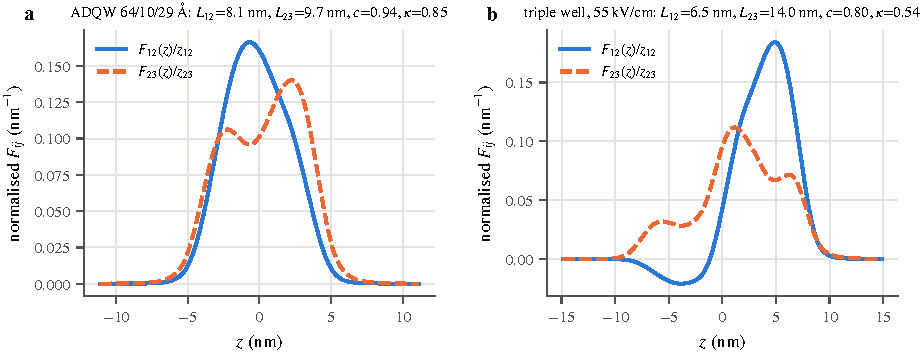
\includegraphics[width=\textwidth]{figures/fig1_geometry.pdf}
\caption{Normalized cumulative transition charges $F_{12}(z)/z_{12}$ (pump transition) and $F_{23}(z)/z_{23}$ (upper ladder transition) at $n_s=10^{12}$~cm$^{-2}$, with effective lengths $L_{ij}$, shape correlation $c$ and $\kappa_\mathrm{exc}=c\sqrt{L_{12}/L_{23}}$ (Proposition~\ref{prop:geom}). (a) ADQW: the two profiles nearly coincide. (b) Triple well, ladder 1--3--4: the upper transition is spread over all three wells and is partly anticorrelated with the pump transition on the left. A single-length effective medium assumes identical profiles ($\kappa=1$).}
\label{fig:geom}
\end{figure}

\paragraph{ADQW and V96 designs.} In the ADQW the two profiles nearly coincide: $L_{12}=8.1$~nm, $L_{23}=9.7$~nm and $c=0.94$, so $\kappa_\mathrm{exc}=0.85$. The two V96 designs and the 50/15/30 control give 0.83--0.87. The permanent-dipole pathway of the ADQW involves a large dipole change, $z_{22}-z_{11}=3.5$~nm, because the electron moves between the wells, and $\kappa_\mathrm{d}=0.95$--0.97.

\paragraph{Triple well.} The TW ladder (states 1, 3 and 4) is different. Its upper transition extends over all three wells ($L_{23}=14.0$~nm), while the pump transition sits in the right-hand well (6.5~nm), and the profiles overlap poorly ($c=0.80$), so $\kappa_\mathrm{exc}=0.54$. Its pump transition also has a large dipole change, $z_{33}-z_{11}=-5.8$~nm, and $\kappa_\mathrm{d}=0.70$--0.71.

\paragraph{Harmonic transition.} In all designs the harmonic transition is more compact than the pump transition: $L_{1n}/L_{12}=0.29$--0.62. A single-length effective medium therefore underestimates its depolarization shift by the same factor.

\section{Collective corrections with only the ground subband occupied}\label{sec:ground}
To isolate the second-order collective physics we first keep three ladder subbands with all electrons in the ground state. This is a model: at $2\times10^{12}$~cm$^{-2}$ the zero-temperature Fermi energy, about 110~meV, already exceeds $E_{12}$. In the ADQW, $\Delta_{12}=3.6$, 7.6, 16.0 and 33~meV at $n_s=0.5$, 1, 2 and $4\times10^{12}$~cm$^{-2}$.

\paragraph{Closed form for $F_\mathrm{exc}$.} Figure~\ref{fig:path}a compares $F_\mathrm{exc}=\tilde U_{32}/qEz_{23}$, evaluated with the full first-order TDH solution, with the closed form of Eq.~\eqref{eq:F}. Over 110--140~meV they agree to within 0.06 in real and imaginary parts up to $10^{12}$~cm$^{-2}$, and to within 0.3 at $2\times10^{12}$~cm$^{-2}$, where coupling to the other coherences grows.

\paragraph{Exact decomposition.} At second order Eq.~\eqref{eq:tdh} is linear in $\tilde U$, so $P^{(2)}$ splits exactly into contributions from the matrix elements of $\tilde U$, each with a bare part and a Hartree part (Table~\ref{tab:decomp}).
\begin{itemize}
\item The Hartree part of the excited-state pathway is in quadrature with the bare part, grows as $\kappa_\mathrm{exc}\Delta_{12}/\gamma$, and raises $|P^{(2)}|$.
\item The Hartree part of the permanent-dipole pathway is real and positive while the total is dominated by a negative real part, so it lowers $|P^{(2)}|$. Physically, the oscillating charge of the 1--2 coherence produces a diagonal Hartree potential at $\omega$, which modulates the 1--2 energy and generates a $2\omega$ coherence.
\end{itemize}
Energy substitution has neither term.

\begin{table}[!t]\centering\small
\caption{Exact decomposition of the peak second-order polarization of the three-level ADQW (ground state only) by the matrix elements of the first-order effective potential that drive it, normalized to the magnitude of the total. ``exc'' is $\tilde U_{23}$, ``diag'' is $\tilde U_{ii}$ and ``rest'' is $\tilde U_{12},\tilde U_{13}$. The Hartree parts are the collective contributions; $F_\mathrm{exc}$ and $F_\mathrm{d}$ are evaluated with the full first-order solution. The last column is the ratio of peak $|\chitwo|$ from TDH to that from energy substitution. $^\dagger$Third state is a resonance above the spacer band edge (box-dependent).}
\label{tab:decomp}
\setlength{\tabcolsep}{2.5pt}\footnotesize
\begin{tabular}{cccccccccc}
\toprule
$n_s$ & $\Delta_{12}$ & $|F_\mathrm{exc}|$ & $|F_\mathrm{d}|$ & exc, bare & exc, Hartree & diag, bare & diag, Hartree & rest & TDH/Ando\\
($10^{12}$~cm$^{-2}$) & (meV) & & & & & & & & \\
\midrule
0.5 & 3.6 & 1.03 & 1.04 & $-1.00+0.03i$ & $+0.03+0.30i$ & $+0.04+0.26i$ & $+0.08-0.02i$ & $-0.03-0.11i$ & 0.99\\
1 & 7.6 & 1.19 & 1.24 & $-0.87-0.07i$ & $-0.08+0.51i$ & $+0.01+0.23i$ & $+0.15+0.00i$ & $-0.05-0.12i$ & 1.11\\
2 & 16.0 & 1.58 & 1.73 & $-0.68-0.07i$ & $-0.16+0.75i$ & $+0.03+0.18i$ & $+0.23-0.00i$ & $-0.10-0.13i$ & 1.38\\
4$^\dagger$ & 33.4 & 1.94 & 2.29 & $-0.63-0.00i$ & $+0.32+1.18i$ & $+0.14+0.17i$ & $+0.29-0.39i$ & $-0.25+0.04i$ & 1.54\\
\bottomrule
\end{tabular}
\end{table}

\paragraph{Kernel blocks.} Table~\ref{tab:masks} isolates the kernel blocks:
\begin{itemize}
\item ``self'': each off-diagonal pair with itself, which produces the Ando shifts;
\item ``cross'': two different off-diagonal pairs, which carries $\kappa_\mathrm{exc}$ and the multisubband coupling;
\item ``diag'': any element involving a diagonal pair, which carries $\kappa_\mathrm{d}$.
\end{itemize}

\paragraph{ADQW.} With the self block only (the $\kappa=0$ limit of Eq.~\eqref{eq:path}) TDH is within 5\% of energy substitution at $10^{12}$~cm$^{-2}$ and 10\% at $2\times10^{12}$~cm$^{-2}$. This difference measures the terms that Eq.~\eqref{eq:path} neglects (non-RWA terms, screening of the nonresonant matrix elements and the coupling of the $2\omega$ coherences). Adding the cross block raises $|\chitwo|$ to 1.24 and 1.60 times the energy-substitution value; adding the diagonal block instead lowers it to 0.88 and 0.79. Together they give 1.11 and 1.38, i.e.\ the enhancement predicted by Załużny's coupling factor \cite{Zaluzny1995} and by local-field arguments \cite{Krieguer2024}, reduced by the opposing diagonal term (as in the benchmark of Sec.~\ref{sec:bench}).

\paragraph{Triple well.} Here the same blocks \emph{lower} $|\chitwo|$, to 0.90 and 0.77 of energy substitution. The cross block alone gives 0.93 and 0.81, because the excited-state and the large permanent-dipole pathways interfere destructively at the operating point: in the TW the bare permanent-dipole contribution opposes the bare excited-state one, while in the ADQW it is in quadrature with it. A factor $|F_p|>1$ therefore does not guarantee enhancement.

\begin{table}[!t]\centering\small
\caption{Peak $|\chitwo|$ from TDH relative to energy substitution, with the kernel restricted to the blocks listed (self: Ando shifts; cross: different off-diagonal pairs; diag: elements with a diagonal pair). ``Ground'': three ladder subbands, all electrons in level 1. ``300~K'': all bound subbands with self-consistent populations; $\rho_\mathrm{lad}$ is the population of the intermediate ladder level (level 2 of the ADQW, level 3 of the TW).}
\label{tab:masks}
\begin{tabular}{llccccccc}
\toprule
Design & populations & $n_s$ ($10^{12}$~cm$^{-2}$) & $\rho_\mathrm{lad}$ & self only & self+cross & self+diag & full\\
\midrule
ADQW & ground & 1 & 0 & 1.05 & 1.24 & 0.88 & 1.11\\
 & & 2 & 0 & 1.10 & 1.60 & 0.79 & 1.38\\
 & 300 K & 1 & 0.035 & 1.04 & 1.18 & 0.89 & 1.05\\
 & & 2 & 0.119 & 1.05 & 1.07 & 0.82 & 0.96\\
TW & ground & 1 & 0 & 1.01 & 0.93 & 0.98 & 0.90\\
 & & 2 & 0 & 1.00 & 0.81 & 0.97 & 0.77\\
 & 300 K & 1 & 0.015 & 1.01 & 0.98 & 0.98 & 0.95\\
 & & 2 & 0.025 & 1.02 & 0.93 & 0.98 & 0.89\\
\bottomrule
\end{tabular}
\end{table}

\section{Self-consistent populations: multisubband coupling}\label{sec:thermal}
\paragraph{Mechanism.} Double resonance requires $E_{23}\approx E_{12}\approx\hbar\omega$. In the ADQW at $2\times10^{12}$~cm$^{-2}$ the collective energies are $\Et_{12}=119.5$~meV and $\Et_{23}=133.9$~meV, both within $1.5\gamma$ of the pump. Any population of level 2 makes the 2--3 transition active at the pump frequency. The kernel element $S_{23,12}$, the same one that sets $\kappa_\mathrm{exc}$, then couples the 1--2 and 2--3 coherences in linear response, forming a multisubband plasmon of the kind observed in absorption \cite{Delteil2012}.

\paragraph{Occupation of level 2.} At $2\times10^{12}$~cm$^{-2}$ the self-consistent population of level 2 is $\rho_2=0.12$ at 300~K. It is still 0.045 at 77~K, because the Fermi level lies near $E_2$, so the occupation is partly thermal and partly degenerate.

\paragraph{Counterfactual test.} The cleanest test keeps the 300~K states and sets $\rho_2=0$ (all electrons in level 1). With the self-consistent populations, the TDH pump-band absorption is a doublet with peaks at 119.5 and 133.5~meV, and $|\chitwo|$ is 0.96 times the energy-substitution value. With $\rho_2=0$ the doublet collapses into a single line at 123.0~meV and the ratio becomes 1.38.

\paragraph{Source and propagation roles.} Removing the $(12)\times(23)$ block either from the second-order source or from the Liouvillian separates its two roles (Fig.~\ref{fig:path}b):
\begin{itemize}
\item \emph{In the source} (the pathway factor) it raises $|\chitwo|$ in every ADQW case, for example from 0.75 to 1.30 times the energy-substitution value at 300~K and $2\times10^{12}$~cm$^{-2}$.
\item \emph{In the Liouvillian}, which contains the multisubband mixing at $\omega$ and the coupling of coherences at $2\omega$, it does nothing when $\rho_2=0$ (77~K, $10^{12}$~cm$^{-2}$). With $\rho_2=0.12$ it lowers the full result from 1.30 to 0.96.
\end{itemize}
The good agreement of energy substitution at $2\times10^{12}$~cm$^{-2}$ and 300~K is therefore a cancellation, not evidence that collective effects are small.

\paragraph{Triple well.} In the TW the intermediate ladder level (level 3) holds at most 2.5\% of the electrons. The low-lying level 2, at 39--44~meV, is heavily populated ($\rho_2=0.25$--0.34) and adds a separate 2--3 line at 82--90~meV. The reduction in Table~\ref{tab:masks} comes mainly from pathway interference (Sec.~\ref{sec:ground}). The level-2 mechanism above is specific to compact two-well ladders whose level 2 lies near the Fermi level.

\begin{figure}[!t]\centering
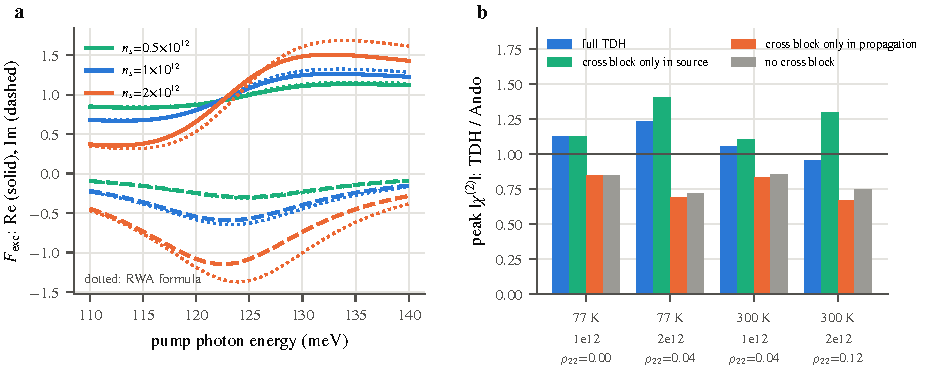
\includegraphics[width=\textwidth]{figures/fig4_pathway.pdf}
\caption{(a) Pathway factor $F_\mathrm{exc}=\tilde U_{32}/qEz_{23}$ of the three-level ADQW (ground state only), evaluated with the full first-order TDH solution (solid: real part; dashed: imaginary part), and the closed form Eq.~\eqref{eq:F} (dotted). (b) Peak $|\chitwo|$ relative to energy substitution for the ADQW with self-consistent populations, with the $(12)\times(23)$ kernel block kept everywhere (full TDH), only in the second-order source, only in the Liouvillian (propagation), or nowhere.}
\label{fig:path}
\end{figure}

\paragraph{Spectra.} Figures~\ref{fig:spectra} and \ref{fig:ratio} show the spectra with self-consistent populations. Up to $10^{12}$~cm$^{-2}$ the peak $|\chitwo|$ from TDH lies within 6\% of energy substitution for all five designs (0.95--1.06). At $2\times10^{12}$~cm$^{-2}$ the deviations are 4--15\%:
\begin{itemize}
\item ADQW: 0.96, through the cancellation above;
\item ADQW 50/15/30: 1.19$^\dagger$;
\item TW: 0.89;
\item V96 SI: 0.91$^\dagger$;
\item V96 WG(DR): 0.85.
\end{itemize}
These deviations do not follow the size of the Ando shift (4.3--5.3~meV in the last three designs), so no simple criterion in $\Delta/\gamma$ separates the cases. At $4\times10^{12}$~cm$^{-2}$, where a coupled mode carries most of the pump-band oscillator strength (and the third ADQW level lies above the spacer band edge, so the values depend on the box), TDH gives 218~nm/V for the ADQW, against 428~nm/V from energy substitution. The LF model follows TDH in the ADQW, where $\kappa\approx1$, but gives 123~nm/V against 153~nm/V in the TW (20\% low), whose $\kappa_\mathrm{exc}=0.54$ and $\kappa_\mathrm{d}=0.71$ are far from the LF assumption, and 114~nm/V against 181~nm/V at $4\times10^{12}$~cm$^{-2}$ (37\% low; at this density the upper TW levels, including a weakly localized fifth state about 250~meV above level 2 that the basis retains, lie above the band edge of the right-hand spacer, so this value depends on the box).

\begin{figure}[!t]\centering
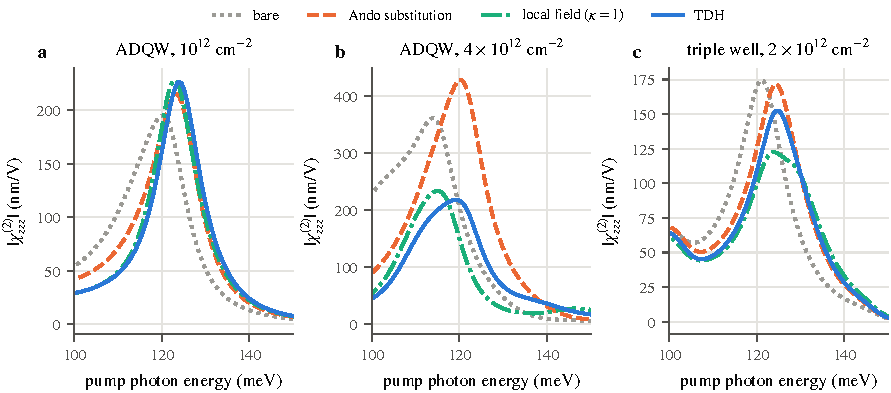
\includegraphics[width=\textwidth]{figures/fig2_spectra.pdf}
\caption{$|\chitwo_{zzz}(2\omega;\omega,\omega)|$ against pump photon energy from the four treatments, with self-consistent populations at 300~K. (a) ADQW, $10^{12}$~cm$^{-2}$: all collective treatments agree to within 6\%. (b) ADQW, $4\times10^{12}$~cm$^{-2}$: energy substitution overestimates the peak by a factor of 2.0. (c) Triple well, $2\times10^{12}$~cm$^{-2}$: the local-field model ($\kappa=1$) underestimates the peak by 20\%.}
\label{fig:spectra}
\end{figure}

\begin{figure}[!t]\centering
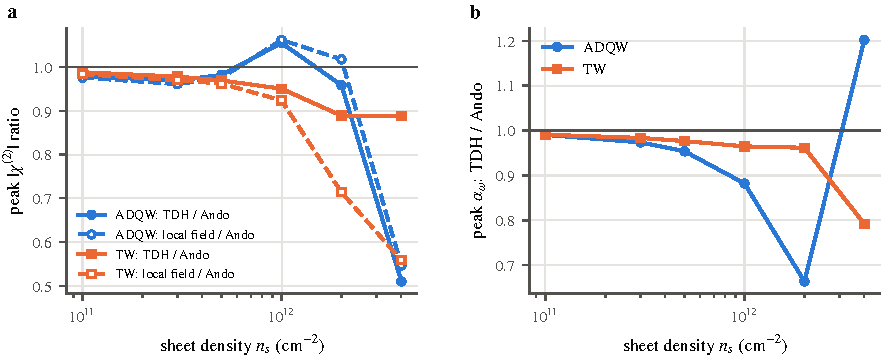
\includegraphics[width=\textwidth]{figures/fig3_ratio.pdf}
\caption{(a) Peak $|\chitwo|$ from TDH (solid) and from the local-field model (dashed) relative to energy substitution, against sheet density, for the ADQW and the triple well at 300~K. (b) Peak pump-band absorption from TDH relative to energy substitution (global maxima within 90--160~meV; the rise at $4\times10^{12}$~cm$^{-2}$ in the ADQW is the upper coupled mode at 142.0~meV).}
\label{fig:ratio}
\end{figure}

\paragraph{Absorption.} The absorption shows the mixing directly (Fig.~\ref{fig:abs}). At $2\times10^{12}$~cm$^{-2}$ the TDH pump-band absorption of the ADQW is a doublet with nearly equal peaks at 119.5 and 133.5~meV. Its maximum, 5030~cm$^{-1}$, is 34\% below the 7570~cm$^{-1}$ that energy substitution places in a single line. At $4\times10^{12}$~cm$^{-2}$ most of the strength sits in an upper mode at 142.0~meV. Because the efficiency depends on $\aw$ as well as on $\chitwo$, this transfer matters as much as the change in $\chitwo$.

\begin{figure}[!t]\centering
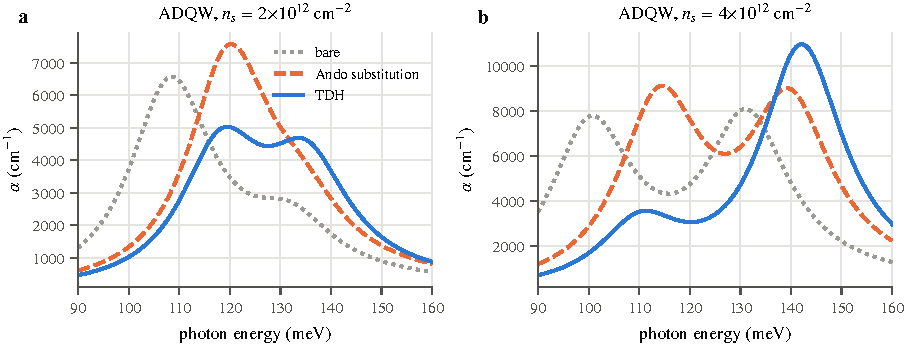
\includegraphics[width=\textwidth]{figures/fig6_absorption.pdf}
\caption{ISB absorption of the ADQW at 300~K from the bare, energy-substitution and TDH treatments (drive-referenced, $n=3.3$). Partial occupation of level 2 lets the depolarization coupling split the pump line into a multisubband-plasmon doublet (a); at $4\times10^{12}$~cm$^{-2}$ most of the strength moves to an upper mode (b).}
\label{fig:abs}
\end{figure}

\section{Efficiency merit across designs}\label{sec:fom}
For a resonant ladder in the small-signal regime, the phase-matched efficiency at the optimum length is \cite{OwnbyNL02}
\begin{equation}
\eta^*\propto M\,I_\omega,\qquad M\equiv g(u)\frac{|\chitwo|^2}{\aw\aww},\qquad g(u)=u^{-(u+1)/(u-1)},\quad u=\frac{2\aw}{\aww},
\end{equation}
where $I_\omega$ is the pump intensity. We evaluate $M$ at the pump energy of maximum $|\chitwo|$, the doubly resonant operating point, from the material absorptions; waveguide losses and modal factors are omitted. We normalize $M$ by its bare value at the same density, which isolates the collective effects. Table~\ref{tab:survey} lists the results.

\begin{table}[!t]\centering\small
\caption{Design survey at 300~K. Ladder: the subbands $m,n$ (ground state 1) with the largest double-resonance-weighted product $|z_{1m}z_{mn}z_{n1}|$. $E_{1m}$ and $E_{1n}$ are self-consistent single-particle energies at the stated density, and ``shift'' is the Ando shift of the pump transition. V96 layer sequences are from Table~I of Ref.~\cite{Vurgaftman1996}; their energies at these densities differ from the flat-band values listed there. $|\chitwo|$ is the peak magnitude from the bare, energy-substitution, local-field and TDH treatments. $M/M_\mathrm{bare}$ is the optimum-length efficiency merit at the $|\chitwo|$ maximum relative to the bare value. $^\dagger$Third state is a resonance above the spacer band edge (box-dependent); these rows are excluded from the ranges quoted in the text.}
\label{tab:survey}
\setlength{\tabcolsep}{3.5pt}
\begin{tabular}{lccccccccc}
\toprule
Design & $n_s$ & ladder & $E_{1m}/E_{1n}$ & shift & $\kappa_\mathrm{exc}$ & $|\chitwo|$ (nm/V) & \multicolumn{3}{c}{$M/M_\mathrm{bare}$}\\
& ($10^{12}$) & & (meV) & (meV) & & bare/Ando/LF/TDH & Ando & LF & TDH\\
\midrule
ADQW 64/10/29 & 1 & 2,3 & 116/244 & 6.8 & 0.85 & 195/215/228/227 & 0.84 & 1.11 & 1.09 \\
 & 2 & 2,3 & 108/240 & 11.6 & 0.86 & 270/347/354/333 & 0.65 & 1.14 & 1.04 \\
TW, 55 kV/cm & 1 & 3,4 & 123/246 & 2.6 & 0.54 & 109/109/101/104 & 0.93 & 0.80 & 0.85 \\
 & 2 & 3,4 & 126/243 & 4.3 & 0.54 & 174/172/123/153 & 0.91 & 0.53 & 0.73 \\
V96 WG(DR) 62/20/29 & 1 & 2,3 & 107/228 & 2.7 & 0.87 & 134/131/133/125 & 0.92 & 0.91 & 0.92 \\
 & 2 & 2,3 & 96/224 & 4.6 & 0.87 & 153/150/141/127 & 0.84 & 0.91 & 0.75 \\
V96 SI 26/19.5/57 & 1 & 2,3 & 119/249 & 3.0 & 0.86 & 139/139/141/135 & 0.92 & 0.94 & 0.95 \\
 & 2$^\dagger$ & 2,3 & 107/245 & 5.3 & 0.86 & 160/161/165/146 & 0.84 & 1.04 & 0.85 \\
ADQW 50/15/30 & 1 & 2,3 & 92/284 & 5.8 & 0.83 & 62/62/65/63 & 0.88 & 1.16 & 1.07 \\
 & 2$^\dagger$ & 2,3 & 86/279 & 9.2 & 0.81 & 98/113/142/135 & 0.69 & 1.65 & 1.44 \\
\bottomrule
\end{tabular}
\end{table}

At the doubly resonant operating point:
\begin{itemize}
\item TDH gives $M/M_\mathrm{bare}$ between 0.73 and 1.09, so the enhancement of $\chitwo$ at the shifted resonance does not raise the merit, because the absorption is enhanced too. An off-resonant control whose third level is a resonance gives up to $+44\%$ (Table~\ref{tab:survey}), but that value depends on the box.
\item Energy substitution can be pessimistic: for the ADQW at $2\times10^{12}$~cm$^{-2}$ it gives 0.65 against 1.04, because it overestimates the pump absorption (Sec.~\ref{sec:thermal}). Elsewhere it differs from TDH by up to 25\%, in either direction.
\item The local-field model is within 10\% of TDH except for the TW at $2\times10^{12}$~cm$^{-2}$, which it underestimates by a factor of 1.36, and the V96 WG(DR) design at that density, which it overestimates by 21\%.
\end{itemize}

These comparisons depend on the operating point. Within $\pm2\gamma$ of the $|\chitwo|$ maximum, $M$ usually keeps rising away from resonance, consistent with the case for detuned pumping in Ref.~\cite{OwnbyNL02}. The best values are then:
\begin{itemize}
\item TDH, 0.58--1.42 of the bare value;
\item for the ADQW at $10^{12}$~cm$^{-2}$, 1.11 from energy substitution against 0.77 from TDH.
\end{itemize}
They mostly lie at the edge of that range, where Lorentzian line wings with constant $\gamma$ are not reliable. For design purposes, collective effects change the merit by tens of percent in either direction, and neither shortcut predicts the sign reliably.

\section{Double counting of the depolarization shift}\label{sec:double}
Absorption measurements give the collective energies $\Et_{ij}$. A common route to a device model adopts these as level spacings, by adjusting the band structure or by inserting them directly, and then describes the doped layer by a local-field or $\varepsilon_{zz}$ model. That applies the depolarization a second time. We emulate this by using the Ando energies as single-particle energies in the LF model:
\begin{itemize}
\item \emph{ADQW, against TDH.} The pump line is placed 7.0~meV (at $10^{12}$~cm$^{-2}$) and 16.8~meV (at $2\times10^{12}$~cm$^{-2}$) too high, and the peak $|\chitwo|$ is 170 and 180~nm/V against 227 and 333~nm/V.
\item \emph{ADQW, against LF with the correct energies}, which isolates the double counting: $-26\%$ and $-49\%$.
\item \emph{TW.} The line shifts by 3.0 and 5.3~meV. Against LF with the correct energies, $|\chitwo|$ changes by $-1\%$ and $+13\%$; against TDH, by $-4\%$ and $-10\%$.
\end{itemize}
Measured collective energies should therefore be used either in energy substitution or as the target for a single-particle band structure that is then fed to a collective model, but not in both places.

\section{Saturation}\label{sec:dynamic}
Under strong pumping the populations change, and with them both the depolarization shifts [Eq.~\eqref{eq:Delta}] \cite{Zaluzny1993,Craig1996,Cominotti2023} and, in an asymmetric structure, the static Hartree potential. For a two-level rectangular well Załużny showed that the depolarization shift falls with intensity and the saturated line becomes asymmetric; he noted that the static field of optically generated space charge also shifts the subbands but is small in rectangular wells \cite{Zaluzny1993}. In an asymmetric double well it is not small: electrons excited to level 2 move to the other well (here $z_{22}-z_{11}=3.5$~nm), and their charge shifts all levels. In Eq.~\eqref{eq:tdh} both effects are contained in the kernel acting on the population changes. The companion saturation study \cite{OwnbyNL02} used rate equations with Ando energies frozen at their equilibrium values.

\paragraph{Models compared.} We integrate Eq.~\eqref{eq:tdh} in real time for the ADQW with its LO-phonon rate matrix and compare $\chitwo_\mathrm{eff}=P_{2\omega}/\varepsilon_0E^2$ and $\aw$ with three models:
\begin{itemize}
\item the frozen-shift rate model;
\item a quasi-static rate model, in which the subband energies follow the saturated populations self-consistently: the states are rediagonalized in the static Hartree potential of the population change, and the Ando shifts are recomputed from the new population differences;
\item a bare control at the same photon energy, real-time without the kernel against bare rate equations, which measures the coherent strong-field corrections that no rate model contains.
\end{itemize}
TDH and the frozen model are each evaluated at their own small-signal $|\chitwo|$ maximum. We also compute the TDH linear absorption about the time-averaged populations of each real-time run, with the static Hartree potential included. This is a linear-response estimate of where the pump-band resonances sit under pumping (Fig.~\ref{fig:dyn}c).

\begin{figure}[!t]\centering
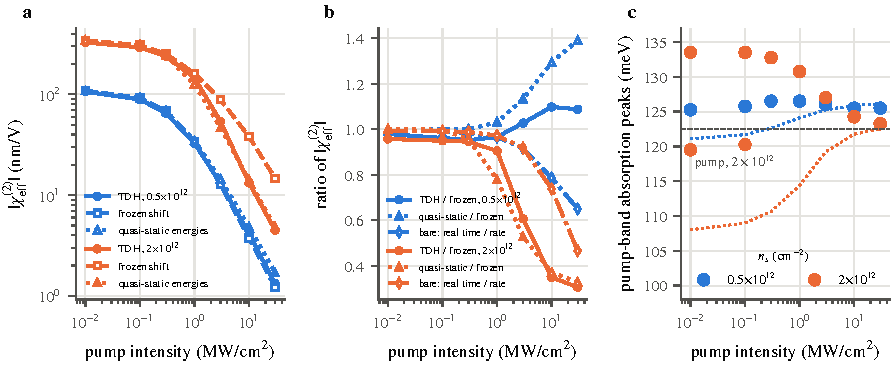
\includegraphics[width=\textwidth]{figures/fig5_dynamic.pdf}
\caption{Saturation of the ADQW (LO-phonon relaxation, $\gamma=10$~meV, 300~K). (a) Effective $|\chitwo|$ against drive intensity from real-time TDH, the frozen-shift rate model of Ref.~\cite{OwnbyNL02}, and the quasi-static rate model whose energies follow the populations (static Hartree potential plus Ando shifts). (b) Ratios to the frozen-shift model, and the bare control (real-time density matrix without the kernel against bare rate equations, at the TDH photon energy). (c) Peaks of the TDH pump-band absorption about the saturated populations (dot size: relative height), and the single-particle $E_{12}$ in the static Hartree potential (dotted); the dashed line marks the pump at $2\times10^{12}$~cm$^{-2}$.}
\label{fig:dyn}
\end{figure}

\paragraph{$2\times10^{12}$~cm$^{-2}$.} The Ando shift is 11.6~meV.
\begin{itemize}
\item In the small-signal regime TDH absorbs 34\% less than the frozen model, because of the multisubband doublet.
\item Above 1~MW/cm$^2$ the absorptions converge, but $|\chitwo|$ from TDH falls to 0.61, 0.35 and 0.31 of the frozen-model value at 3, 10 and 30~MW/cm$^2$.
\end{itemize}
Up to 3~MW/cm$^2$ the quasi-static model reproduces the real-time $|\chitwo|$ to within 14\% (0.86--1.05 of TDH). In this range the reduction is therefore a population-driven shift of the energies, not a coherent collective effect. The quasi-static model does not reproduce the small-signal absorption (1.5 times TDH), because it has no multisubband doublet.

The dominant term is the static Hartree potential of the transferred electrons:
\begin{itemize}
\item It raises the single-particle $E_{12}$ from 108 to 120 and 123~meV at 3 and 30~MW/cm$^2$, while the shrinking depolarization shift moves $\Et_{12}$ only from 119.5 to 123~meV.
\item At the same time $\Et_{13}$ moves from 248 to 245~meV, and the single-particle $E_{23}$ falls from 132 to 121~meV, so the 2--3 transition is pulled onto the pump.
\end{itemize}
The two population terms of $\chitwo$ are $A=(\rho_1-\rho_2)/D_{12}$ and $B=(\rho_2-\rho_3)/D_{23}$. In the frozen model $\Et_{12}$ sits below the pump and $\Et_{23}$ above it, so the terms add: $|A-B|/|A|=0.96$, 1.09 and 1.16 at 3, 10 and 30~MW/cm$^2$. With the shifted energies they partly cancel: $|A-B|/|A|=0.47$, 0.39 and 0.38. The ratio of these brackets, 0.54, 0.41 and 0.37, accounts for almost all of the quasi-static/frozen difference in $|\chitwo|$ (0.53, 0.37 and 0.33).

The probe spectra show the same evolution: the doublet at 119.5 and 133.5~meV merges into a single line that moves from 133 to 123~meV between 0.3 and 30~MW/cm$^2$.

Above 3~MW/cm$^2$ the picture is less complete. At 10 and 30~MW/cm$^2$ the quasi-static model still agrees with TDH (1.06 and 1.07), although it lacks the coherent strong-field corrections measured by the bare control (0.74 and 0.47, where $2qEz_{12}$ reaches 10 and 17~meV, above $\gamma$). Including them would give 0.78 and 0.50 of TDH. A factor of up to about 2 is therefore unresolved in this range, presumably collective terms that offset the coherent corrections.

Both TDH and the quasi-static model screen the static charge-transfer field with the optical background $\varepsilon_b$. With a static permittivity of 13.5 the shift at 30~MW/cm$^2$ falls from 14.6 to 12.5~meV, and the quasi-static $|\chitwo|$ rises by 11--22\%. It remains 0.37--0.64 of the frozen value at 3--30~MW/cm$^2$, so the conclusion survives.

\paragraph{$5\times10^{11}$~cm$^{-2}$, the density of Ref.~\cite{OwnbyNL02}.} The same effects are about three times weaker: the static potential raises $E_{12}$ by up to 5~meV, and the absorption peak moves by less than 1.5~meV. TDH and the frozen model agree to within 5\% in $|\chitwo|$ up to 3~MW/cm$^2$ and within 10\% up to 30~MW/cm$^2$, and to within 5\% in $\aw$ throughout. Above 3~MW/cm$^2$ this agreement involves compensating corrections. The quasi-static energies raise $|\chitwo|$ by 13--39\% at 3--30~MW/cm$^2$, while the coherent corrections of the bare control lower it by 8--35\%; their product, 1.04--0.90, matches the TDH/frozen ratio of 1.03--1.10 to within 17\%. The frozen-shift results of Ref.~\cite{OwnbyNL02} are therefore accurate to about 10\% at this density, but partly through cancellation at the highest intensities.

\paragraph{Consequence.} In asymmetric ladders the pump-induced charge transfer is the main correction to frozen-shift saturation models at high density. It can be included cheaply by updating the Hartree potential with the rate-equation populations. Because it moves the resonances, the photon energy that maximizes the saturated efficiency also moves. Detuned operation \cite{OwnbyNL02} should therefore be optimized with the energies updated, which we have not done here.

\section{Discussion}\label{sec:disc}
\paragraph{Practical guidance.}
\begin{itemize}
\item For the designs studied here, energy substitution gives the peak $|\chitwo|$ to within 6\% up to $10^{12}$~cm$^{-2}$. At the doubly resonant operating point the pump absorption is within 14\%, but the efficiency merit can differ by up to 23\%. It is a reasonable default, provided measured energies are not also passed through a local-field model.
\item Beyond that density, or when a level of the ladder is partly occupied, a self-consistent second-order calculation is needed. The geometric numbers $\kappa_\mathrm{exc}=c\sqrt{L_{12}/L_{23}}$, $\kappa_\mathrm{d}$ and $L_{1n}/L_{12}$ indicate how far a single-length effective medium (a single-Lorentzian $\varepsilon_{zz}$) can be trusted: only when all are close to 1.
\item Collective enhancement of $\chitwo$ does not translate into a higher merit, because the absorption is enhanced too. Pathway interference can turn the enhancement into a reduction (TW).
\item Partial occupation of the intermediate level of a doubly resonant ladder, thermal or degenerate, couples the near-degenerate resonances into multisubband plasmons. This is a further reason, besides the two given by Krieguer and Todorov with only the ground subband occupied (the collective energies define the double resonance, and polaritons in strongly coupled cavities), why single-particle double resonance is not the right target at high density \cite{Krieguer2024}.
\end{itemize}

\paragraph{Relation to previous work.}
\begin{itemize}
\item Załużny's three-level RPA theory \cite{Zaluzny1995} already contains the excited-state factor $F_\mathrm{exc}$, as his $c(\omega)$ with $\kappa_\mathrm{exc}=\bar\alpha_{32}/\alpha_{22}$, and identifies energy substitution as its diagonal approximation ($\kappa=0$). It keeps only the near-resonant $2\omega$ coherence and the ground-state population. It therefore has neither the permanent-dipole Hartree terms nor the multisubband mixing that dominates with level 2 occupied. Our solver reproduces his numbers (Sec.~\ref{sec:bench}).
\item The excited-state factor $F_\mathrm{exc}$ is the planar, leading-order form of the dressed dipoles of Krieguer and Todorov \cite{Krieguer2024}, whose overlap-coupled formalism contains the same $c$ and $L_{ij}$. Their treatment averages away the static (diagonal) terms. Our solver reproduces their three-subband design shift and gives 2.4 for the collective enhancement they put at almost 3 (Sec.~\ref{sec:benchkt}). In a planar stack the Hartree part of these terms contributes 9--23\% of $|P^{(2)}|$ in the ADQW up to $2\times10^{12}$~cm$^{-2}$ (49\% at $4\times10^{12}$~cm$^{-2}$, where the third level is a box-dependent resonance above the spacer band edge) and opposes the excited-state enhancement.
\item The intensity dependence and removal of the depolarization shift were studied in absorption \cite{Zaluzny1993}, observed \cite{Craig1996} and treated in a coherent theory \cite{Cominotti2023}. Załużny noted the static space-charge shift but found it small in rectangular wells \cite{Zaluzny1993}; in the asymmetric double well of Sec.~\ref{sec:dynamic} it outweighs the change of the depolarization shift. The screened harmonic resonances of Heyman \emph{et al.}\ \cite{Heyman1994} are the linear-response physics of Secs.~\ref{sec:ground}--\ref{sec:thermal}.
\end{itemize}
What this paper adds is:
\begin{itemize}
\item a solver without the rotating-wave and near-resonance approximations, benchmarked against Załużny's results;
\item the mapping of the effective-medium (full-wave $\varepsilon_{zz}$) shortcut onto $\kappa=1$, alongside the known $\kappa=0$ limit of energy substitution, and the geometric form of $\kappa_\mathrm{exc}$;
\item the diagonal-kernel (permanent-dipole) pathway in planar structures, which reduces the enhancement in Załużny's own example by 11\%;
\item the identification and counterfactual test of the intermediate-level mechanism in real double-well ladders;
\item a quantitative design survey including the efficiency merit;
\item the double-counting error;
\item the identification, with controls, of pump-induced charge transfer as the main correction to frozen-shift saturation models.
\end{itemize}

\paragraph{Limitations.}
\begin{itemize}
\item The kernel is Hartree only. Exchange and correlation reduce the depolarization shift by an excitonic term, so the time-dependent local-density approximation would give a smaller $\Delta$ at the same density.
\item The linewidth is a constant $\gamma$, and conclusions that depend on line wings (the off-resonant merit) are correspondingly uncertain.
\item In-plane nonparabolicity is not included in the dynamics. In the ADQW the in-plane masses of subbands 1 and 2 differ by 16\%, which spreads $E_{12}$ by 14~meV across the zero-temperature Fermi sea at $2\times10^{12}$~cm$^{-2}$, comparable to $\Delta$ and $\gamma$. Depolarization is known to lock such distributions into a single collective line \cite{Warburton1996}, but a quantitative treatment needs $k$-resolved TDH.
\item The kernel uses a uniform background permittivity across the well and barrier layers, and the same value for the static charge-transfer field under saturation, where the static permittivity would apply (Sec.~\ref{sec:dynamic}).
\item The drive is the displacement field, which makes periods independent. Finite stacks in resonators need the full electromagnetic problem. Under the operating bias the upper ladder levels of the TW lie above the potential at the downhill end of the period (level 4 by 72~meV at $2\times10^{12}$~cm$^{-2}$), so they are quasi-bound, and field-assisted escape, which the single-period model omits, would add to their broadening.
\item The subband states come from a one-band nonparabolic model.
\end{itemize}

\section{Conclusions}
The self-consistent second-order response of a doped ladder can be organised by pathway. To leading order each pathway carries a factor $F_p=1-\kappa_p\Delta_{12}/(\Et_{12}-\hbar\omega-i\gamma)$, where $\kappa_p$ is a ratio of Hartree overlaps of cumulative transition charges. Energy substitution and the single-length effective medium correspond approximately to $\kappa=0$ and $\kappa=1$. For the excited-state pathway $\kappa_\mathrm{exc}=c\sqrt{L_{12}/L_{23}}$ with $|c|\le1$, which is 0.83--0.87 for the double wells studied and 0.54 for a coupled triple well; the permanent-dipole pathway has its own $\kappa_\mathrm{d}$.

The main results are:
\begin{itemize}
\item With only the ground subband occupied, the collective terms raise $|\chitwo|$ in a double well (by 11\% and 38\% at $10^{12}$ and $2\times10^{12}$~cm$^{-2}$) and lower it in the triple well, through pathway interference.
\item In the double well, partial occupation of level 2 couples the near-degenerate 1--2 and 2--3 resonances into a doublet that cancels the enhancement.
\item At the doubly resonant operating point, the efficiency merit changes by $-27\%$ to $+9\%$ up to $2\times10^{12}$~cm$^{-2}$, and the shortcuts err by up to a factor of 1.6.
\item Using measured energies inside a local-field model counts the depolarization twice and costs up to 49\% in $|\chitwo|$.
\item Under saturation at $2\times10^{12}$~cm$^{-2}$, the static Hartree field of pump-transferred electrons pulls the 1--2 and 2--3 resonances onto the pump, and $|\chitwo|$ falls to one third of the frozen-shift value. A rate model with population-dependent energies reproduces this to within 14\% up to 3~MW/cm$^2$. At $5\times10^{11}$~cm$^{-2}$ the frozen-shift model holds to within 10\%.
\end{itemize}

\section*{Data and code availability}
The \texttt{qwkit} software package (v0.7.0) is archived at \url{https://doi.org/10.5281/zenodo.23444120}. The simulation scripts, raw JSON datasets, and figure-generation code that reproduce every result in this study are permanently archived at \url{https://doi.org/10.5281/zenodo.23444568}.

\bibliographystyle{unsrtnat}
\bibliography{refs}
\end{document}
